

\chapter{System Operations}
\label{sec:System Operations}

As mentioned in section \ref{sec:System Overview}, an \ac{ssc} has 32 execution lanes allowing the simultaneous processing of up to 32 \acp{an}.
When processing a group of \acp{an} the basic operations to determine their states are:
\begin{outline}
  %\lbbcleanspace{20pt}
  \lbbcleanspace
  \1 manager streams the states of the pre-synaptic \acp{an} to the \ac{pe}
  \1 manager streams the weights of the pre-synaptic connections to the \ac{pe}
  \1 each execution lane in the \ac{pe} operates directly on the two argument streams using the \ac{stop} block
  \1 the \ac{pe} \ac{simd} block takes the 32 results from the \ac{stop} block and performs the activation function to generate the \ac{an} states
  \1 the \ac{pe} \ac{simd} packetizes the \ac{an} states and sends the packet to the manager
  \1 the manager replicates the \ac{an} state data over the \ac{noc} to any dependent \acp{ssc}
  \1 if the local \ac{ssc} is dependent on the result, the manager saves the \ac{an} state data in local \ac{ssc} \ac{dram}
\end{outline}

This work has developed an instruction architecture to describe the above operations along with other system management operations.
The manager is responsible for instruction decode and coordinating the various data flows and configuration of the modules throughout the \ac{ssc}.
The \ac{pe} is responsible for the main algorithm operations using a combination of its \ac{stop} and \ac{simd} blocks.

\iffalse

The managers primary responsibility is to decode instructions and descriptors and :

\begin{outline}
    \1 Instruction decode
    \1 Internal Configuration messages
    \1 Operand read
    \1 Result write
    \1 Host to \ac{ssc} and \ac{ssc} to \ac{ssc} communication
\end{outline}


The \ac{pe} has three major blocks:

\begin{outline}
    \1 Streaming operation function (\ac{stop})
      \2 Processes data from the manager on-the-fly without storing in local \ac{sram}
    \1 \ac{simd}
      \2 processes the data from the \ac{stop} before returning data to the manager
    \1 DMA/local memory controller
      \2 transfer configuration data to \ac{pe} controller or to store \ac{stop} results to a small local \ac{sram} which can be used for access by \ac{simd} or by the \ac{stop} function
\end{outline}

\fi
% ----------------------------------------------------------------------------------------------------
% ----------------------------------------------------------------------------------------------------
\section{Instructions}
\label{sec:Instructions}

% ----------------------------------------------------------------------------------------------------
%\subsection{Instructions}
%\label{sec:Instructions}
There are two instruction types currently defined, a configuration instruction and a compute instruction.
The configuration instruction has been defined to deal with data downloads and uploads which includes \ac{ann} parameters and input, \ac{ssc} instructions, \ac{simd} and \ac{stop} operation pointers and \ac{simd} instructions.\\
The compute instruction has been defined to deal with computing the states of a group of \acp{an}. \par
\iffalse
\begin{outline}
  \lbbcleanspace
   \1 \ac{ann} parameters and input
   \1 \ac{ssc} instructions
   \1 \ac{simd} and \ac{stop} operation pointers
   \1 \ac{simd} instructions
\end{outline}
Typically an instruction contains information to process a group of \acp{an} but there are other instruction types to synchronize.
A group can be anywhere from one to 32 \acp{an} and is based on the number of execution lanes in the \ac{ssc} (see section \ref{sec:Processing a group of ANes}) and how the user partitions the \ac{ann} across the available \acp{ssc}.
\fi

The instructions contain sub-instructions called descriptors. 
The instruction is an n-tuple where the tuple elements are descriptors and the number of descriptors can vary based on the operation being performed. 
The descriptors contain the details on how to complete the tasks associated with an instruction.
These descriptors are decoded and used to configure the various functions in the \ac{ssc} that will take part in completing the instruction. 
The contents of a single descriptor may be sent to multiple functions and in some cases the manager doesnt parse the contents of the descriptor but immediately passes it to a dependent function.
This allows the system to concurrently prepare for the tasks involved with the instruction.

This works focus has been on the compute instruction as it has the most influence on system performance.
The other instructions have been defined to provide an extensible system for future work.

\subsection{Compute Instruction}
\label{sec:Compute Instruction}

The compute instruction typically contains four descriptors for configuring the tasks associated with processing a group of \acp{an}.
The instruction can be seen in figure \ref{fig:Instruction (4-tuple example)} and includes: 
\begin{itemize}
  %\lbbcleanspace
  \item Operation descriptor containing:
    \begin{itemize}
      \item \ac{stop} operation
      \item \ac{simd} operation
      \item Number of active lanes
      \item Operand Vector length
    \end{itemize}
  \item Two memory read descriptors containing:
    \begin{itemize}
        \item addresses for the pre-synaptic \ac{an} states and connection weights for the two argument streams to the \ac{pe}
        \item how the read data is multiplexed to the execution lanes (broadcast/vectored)
    \end{itemize}
  \item Memory write descriptor containing:
    \begin{itemize}
      \item \ac{dram} address for \ac{an} states
    \end{itemize}
\end{itemize}

\begin{figure}[!t]
\centering
\captionsetup{justification=centering}
\captionsetup{width=.9\linewidth}
\centerline{
\mbox{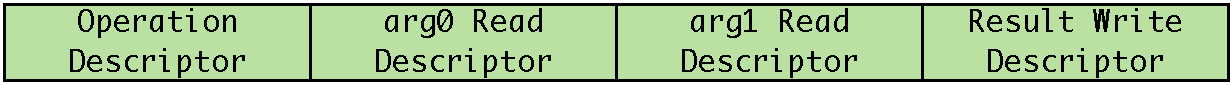
\includegraphics[width=.9\linewidth]{instruction4Tuple}}
}
\caption{Typical compute instruction (4-tuple)}
\label{fig:Instruction (4-tuple example)}
\end{figure}


The descriptor also employs an n-tuple format where the first tuple element always describes the descriptor operation followed by an m-tuple whose elements contain the options required by the operation.
The option elements within a descriptor are a two-tuple with option and associated value and are referred to as option tuples.
These option tuples include a type and value which contain information such as storage descriptor pointer (see section \ref{sec:Storage Descriptor}), \ac{pe} operations and the number of operands.
The length of the value field is currently eight bits or 24-bits. The 24-bit value field is freferred to as an extended tuple and is currently used for memory address and number of operands.
In figure \ref{fig:descriptorTuple} we see the format of a 5-tuple operation descriptor and a list of option types are shown in table \ref{tab:Option tuple functions}.
It should be noted that not all option tuple type are currently used in the system but were provided for expansibility.

\iffalse
\begin{figure}[!t]
\centering
\captionsetup{justification=centering}
\captionsetup{width=.9\linewidth}
\centerline{
\mbox{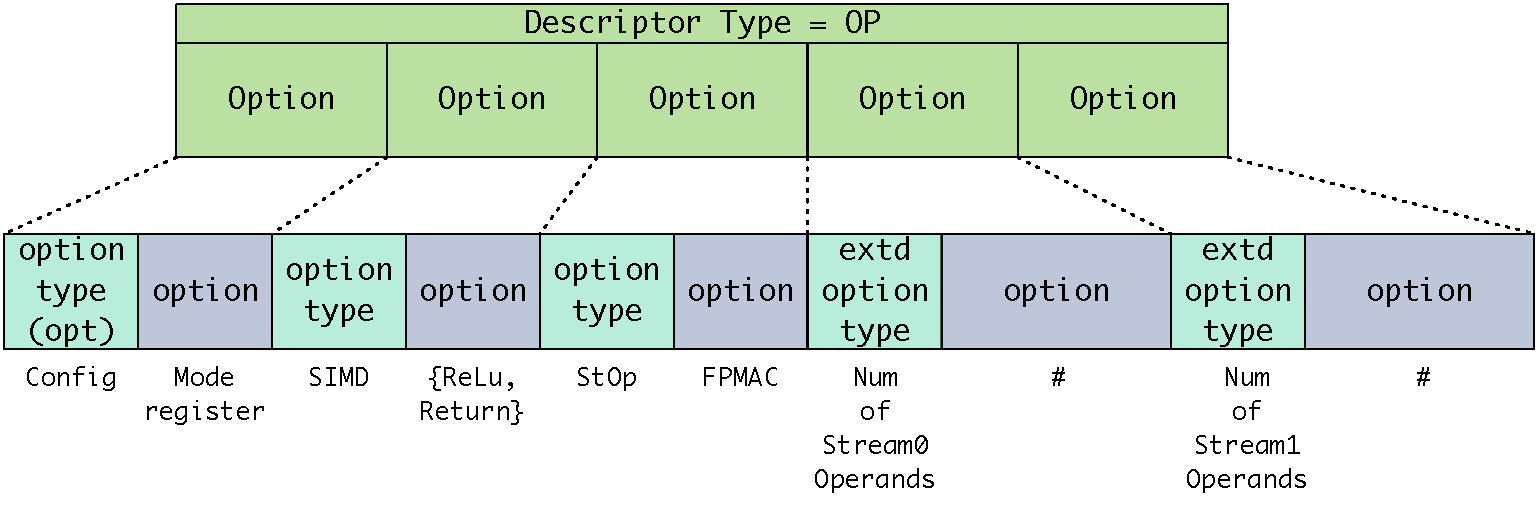
\includegraphics[width=.9\linewidth]{descriptorTuple}}
}
\caption{Operation descriptor (5-tuple example)}
\label{fig:descriptorTuple}
\end{figure}
\fi


\begin{figure}[!t]
  % the [] contains position info e.g. [!t] means here
  \centering
  \captionsetup{justification=centering}

  \begin{minipage}{1\textwidth}
    \centering
    \begin{minipage}{0.85\textwidth}
      \centering
      \captionsetup{justification=centering}
      \captionsetup{width=.9\linewidth}
      \centerline{
      \mbox{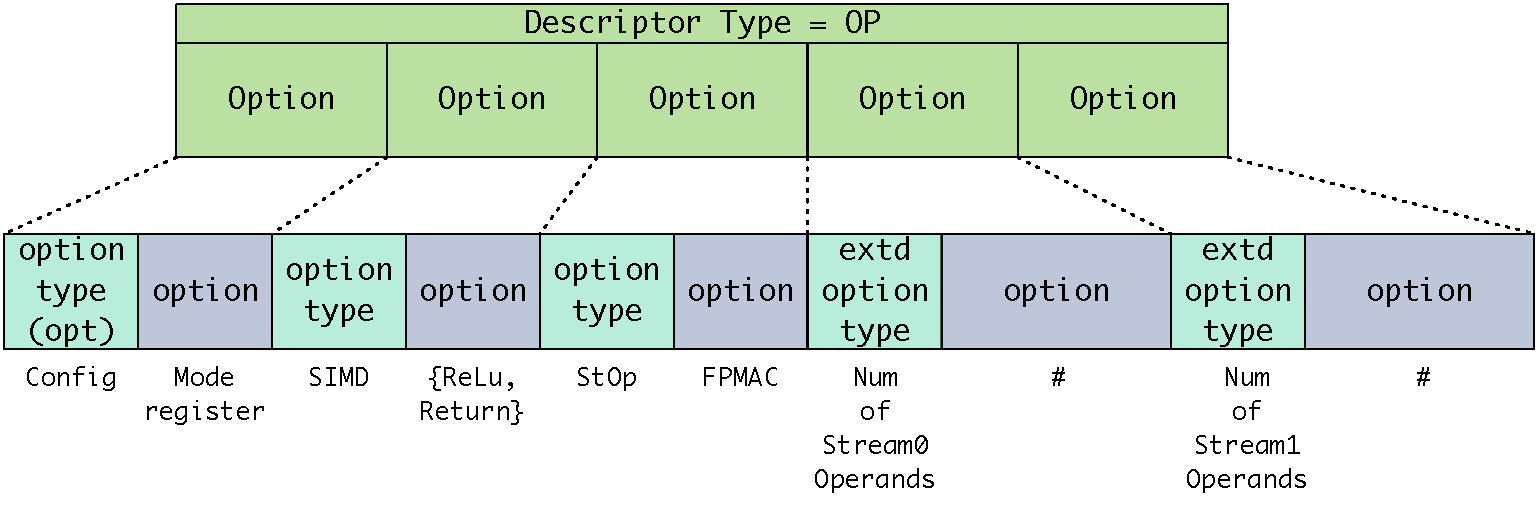
\includegraphics[width=.9\linewidth]{descriptorTuple}}
      }
      \vspace{-2mm}
      \caption{Operation descriptor (5-tuple example)}
      \label{fig:descriptorTuple}
    \end{minipage}
    \begin{minipage}{0.85\textwidth}
        \vspace{5mm}
        \begin{adjustbox}{width=1\textwidth}
            \footnotesize
            \begin{tabular}{ |c|c|c|c|  }
              \hline
              \rowcolor{gray!50}
              \multicolumn{4}{|c|}{Source} \\
              \hline
              \rowcolor{gray!25}
              Type & Type Code & extd &  Value Description  \\
              \hline
              NOP                              &    0   &  N&  \acl{nop} \\
              source                           &    1   &  N&  Used to define the source of any data, such as memory or \ac{pe}  \\
              target                           &    2   &  N&  Used to define the target for any data, such as memory or \ac{pe}  \\
              transfer type                    &    3   &  N&  How data will be directed, vector or braodcast                    \\
              number of lanes                  &    4   &  N&  number of active execution lanes used in opration \\
              \ac{stop} pointer                &    5   &  N&  pointer to \ac{pe} \ac{stop} operation table in \ac{pe} controller \\
              \ac{simd} pointer                &    6   &  N&  pointer to \ac{pe} \ac{simd} instruction memory  \\
              Memory storage descriptor        &    7   &  Y&  pointer to storage descriptor used in memory read or write \\
              num of arg0 operands             &    8   &  Y&  number of operands sent to execution lane stream 0\\
              num of arg1 operands             &    9   &  Y&  number of operands sent to execution lane stream 1\\
              config                           &   10   &  N&  configuration data \\
              status                           &   11   &  N&  status information \\
              \hline
            \end{tabular}
        \end{adjustbox}
        \caption{Option tuple functions}
        \label{tab:Option tuple functions}
    \end{minipage}
  \end{minipage}
\end{figure}


To pull it all together, in figure \ref{fig:Instruction Details} is shown a four-tuple compute instruction with details shown for each of the descriptors.
In figure \ref{fig:Instruction and Descriptors} shows the compute instruction which contains three 4-tuple and one 5-tuple descriptors.
The memory write descriptor shows two storage option elements which indicates the resulting \ac{an} states need to be saved in the memory of two \acp{ssc}.
In figure \ref{fig:Instruction memory waveform} shows the instruction as it is read out of the managers instruction memory and an example of the common interface sugnalling described in section \label{sec:Common Bus Signalling}.
The signals \texttt{wum\textunderscore\textunderscore wud\textunderscore\textunderscore icntl} and \texttt{wum\textunderscore\textunderscore wud\textunderscore\textunderscore dcntl} are used to delineate the instruction and descriptors respectively.
The instruction memory transfers three descriptor elements per cycle which can be seen on the buses \texttt{wum\textunderscore\textunderscore wud\textunderscore\textunderscore option\textunderscore type} and \texttt{wum\textunderscore\textunderscore wud\textunderscore\textunderscore option\textunderscore value}.
\\
Note: The signal name convention used between blocks in the \ac{rtl} use <src>\textunderscore\textunderscore <dest>\textunderscore\textunderscore <signal\textunderscore\textunderscore  name>. In figure \ref{fig:Instruction memory waveform},~ \texttt{wum} and \texttt{wud} refer to "work unit memory" and "work unit decode"
which correspond to the manager instruction memory and instruction decoder respectively.

\begin{figure}
\centering
  \begin{subfigure}{.95\textwidth}
    \centering
    \mbox{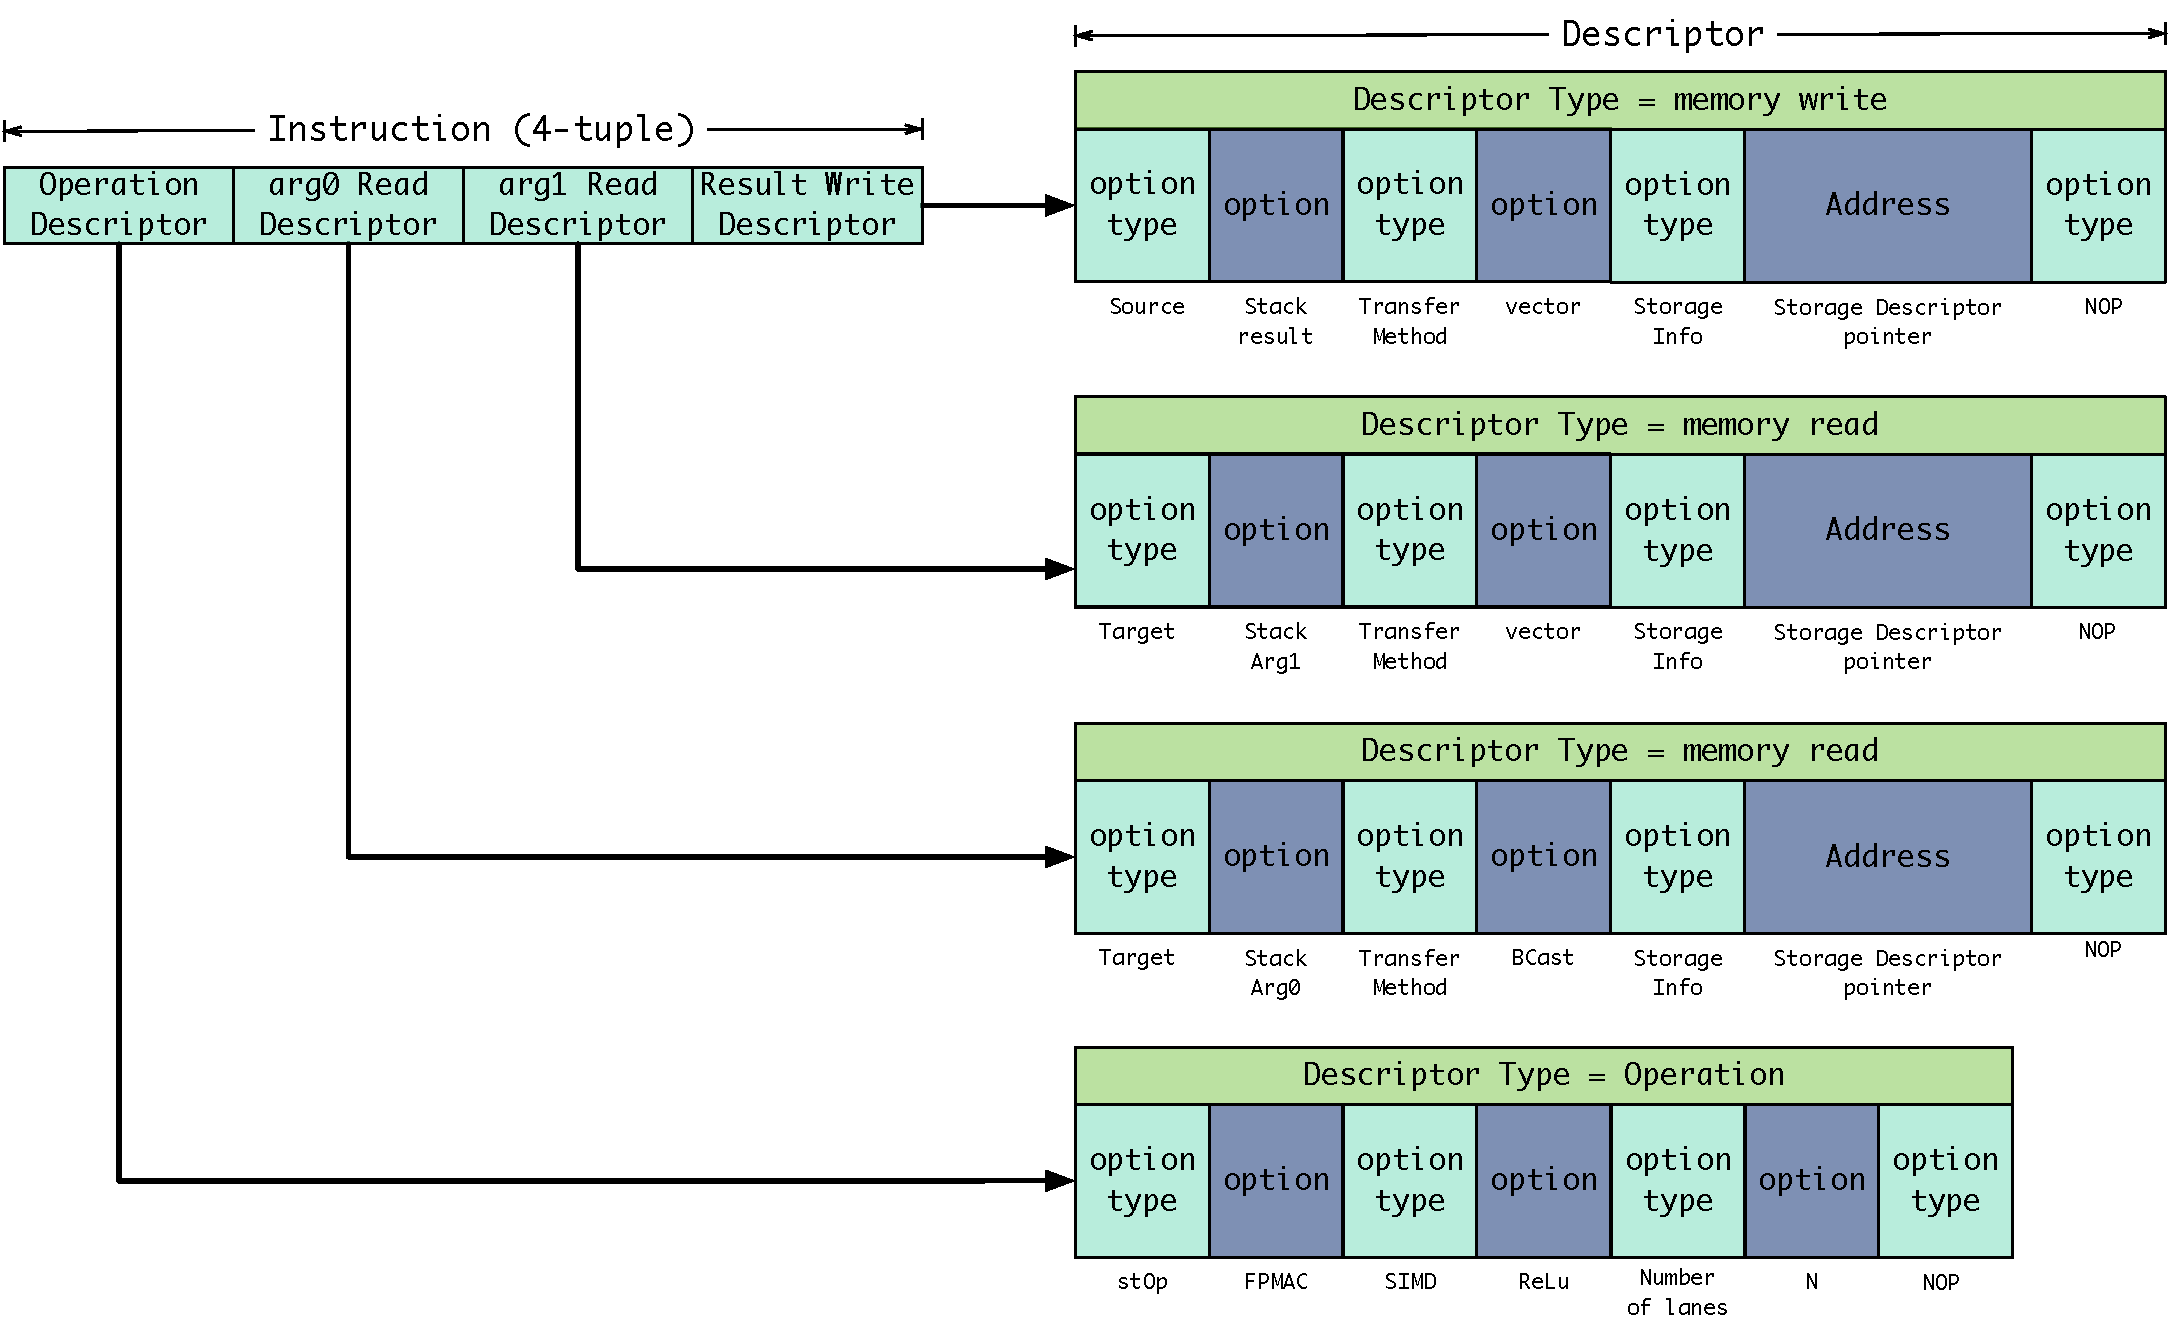
\includegraphics[width=1\linewidth]{instructionAndDescriptors}}
    \captionsetup{justification=centering, skip=6pt}
    \caption{Compute instruction and descriptors}
    \label{fig:Instruction and Descriptors}
  \end{subfigure}%

\bigskip

  \vspace{-35pt}
  \begin{subfigure}{1\textwidth}
    \centering
    \vspace{40pt}
    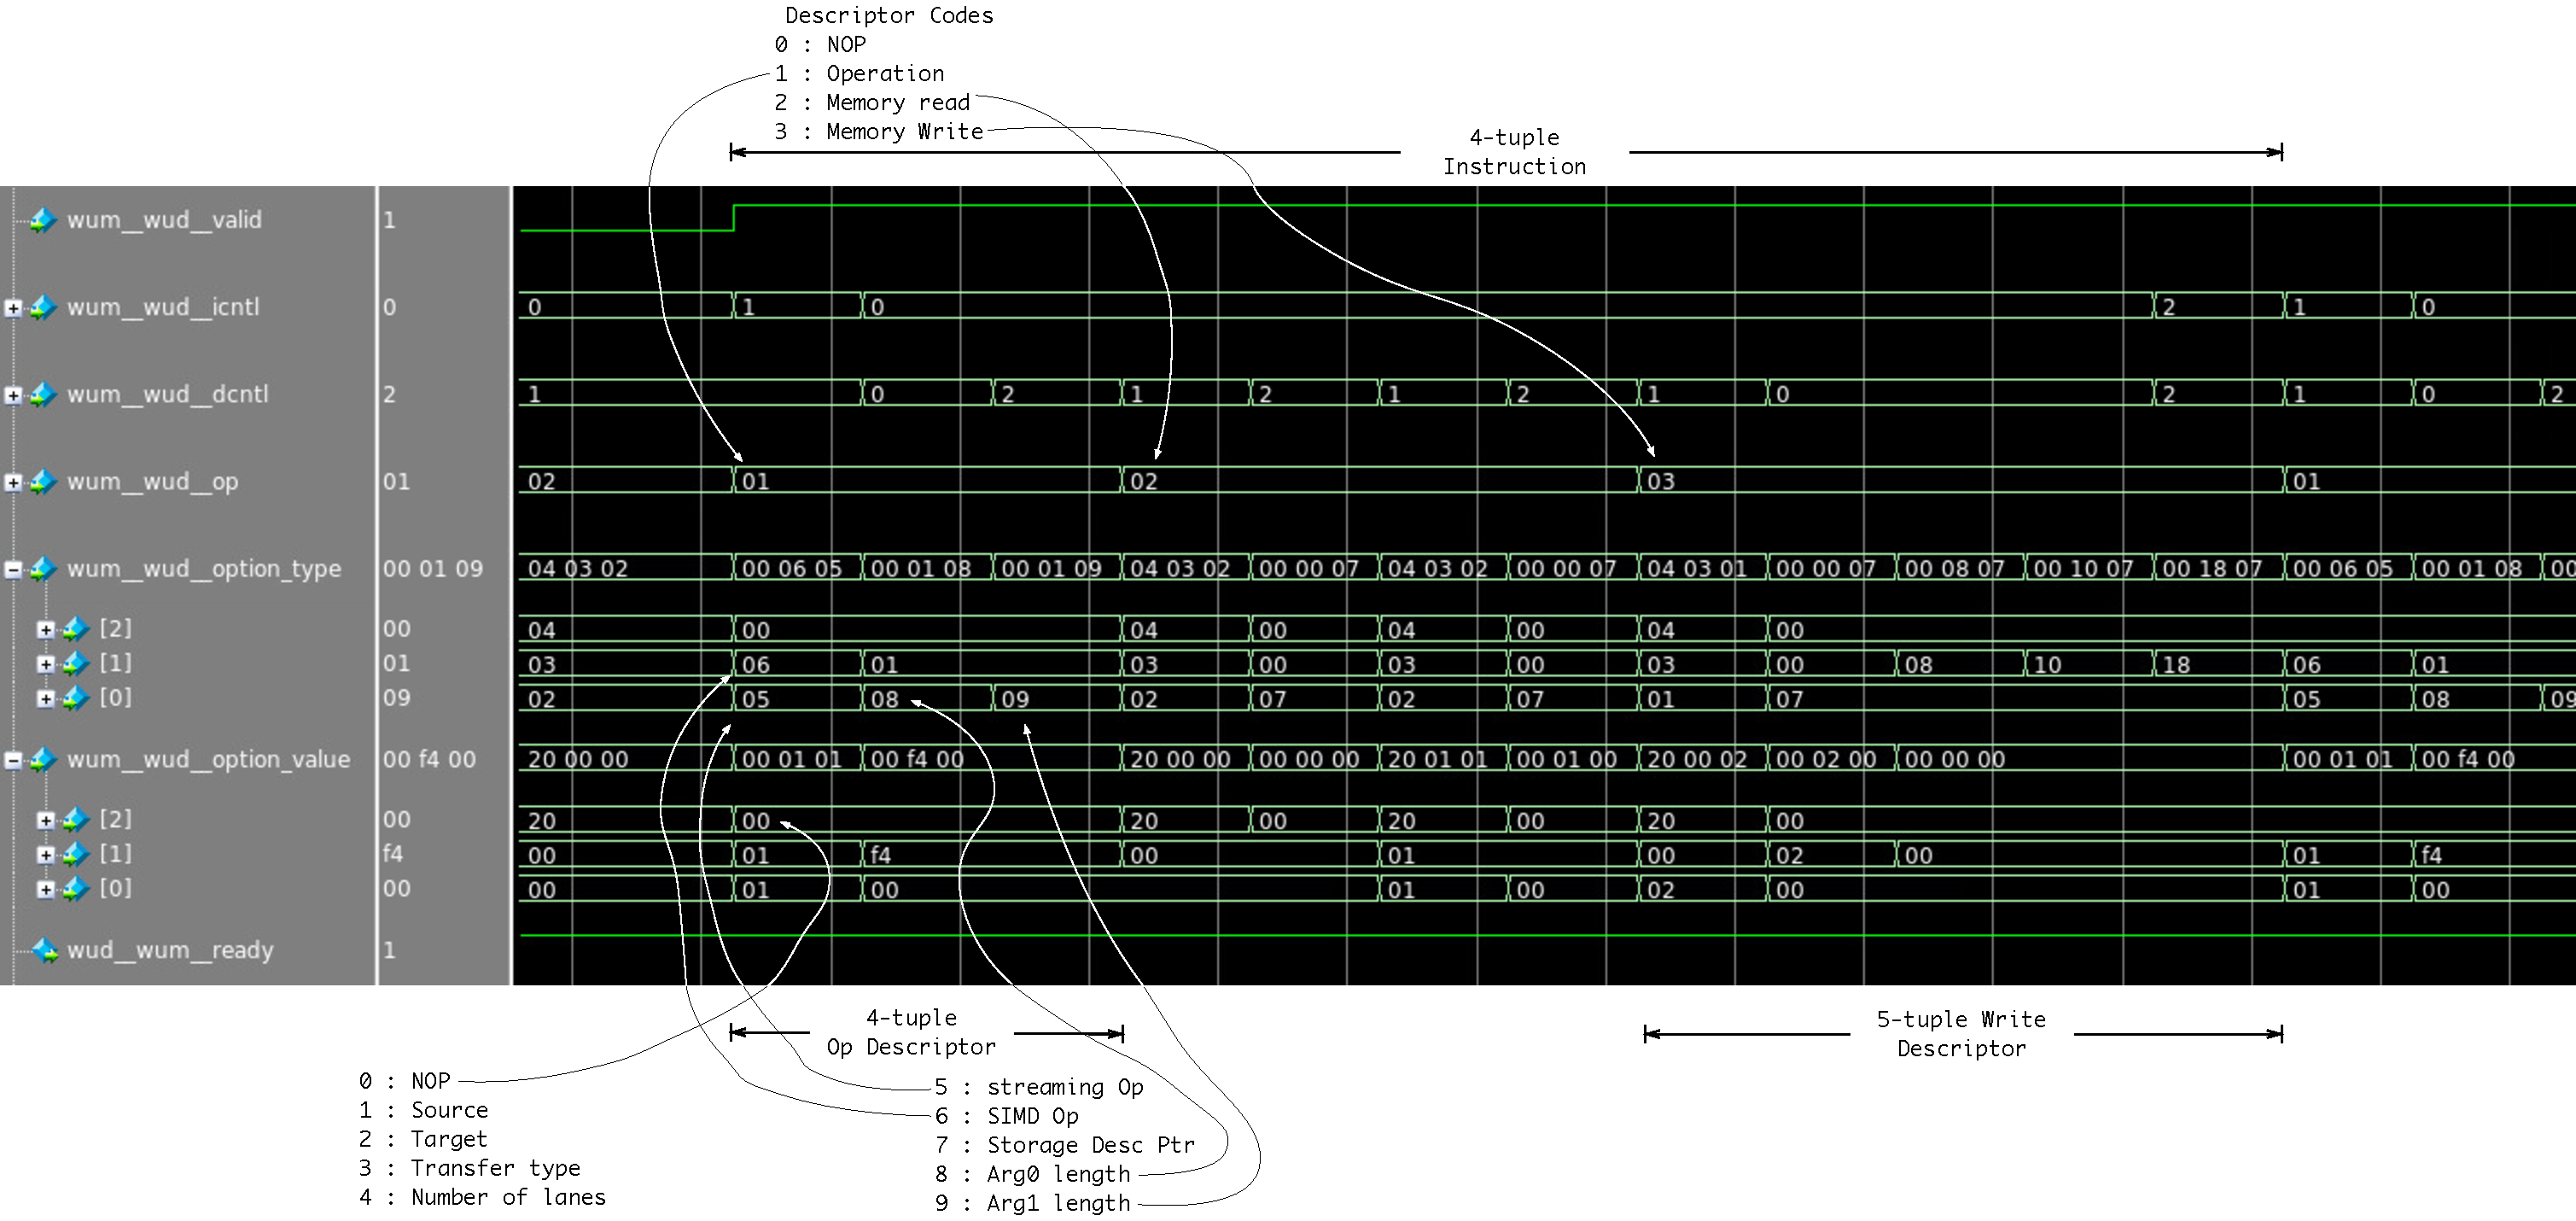
\includegraphics[width=1\textwidth]{instructionWaveform}
    \captionsetup{justification=centering, skip=10pt}
    \caption{Instruction memory waveform}
    \label{fig:Instruction memory waveform}
  \end{subfigure}%
%\vspace{-10pt}
\captionsetup{justification=centering, skip=16pt}
\caption{Compute Instruction details}
\label{fig:Instruction Details}
\end{figure}



% ----------------------------------------------------------------------------------------------------
\subsubsection{Accessing of Pre-synaptic \ac{an} states and connection weights}
\label{sec:AccessingANStates}

A part of the research is determining how to store the \ac{ann} input and parameters in such a way to effectively make use of main \ac{dram} bandwidth. 

To provide parameters for the up to 32 execution lanes within the \ac{pe}, the \ac{an} parameters were stored in consecutive address locations. 
With one read to the \ac{dram}, we access 128 words. This provides four weights for each of the 32 \acp{an} being processed. 
These weights are sent to each lane of the \ac{pe} over four cycles. 
We will discuss memory efficiency later, but by taking advantage of the multiple \ac{dram} banks along with pre-fetching and buffering, we are able to achieve relatively high efficiency of the available maximum bandwidth.

Although \ac{an} parameters (weights) are stored in contiguous memory locations, providing the input state to a particular \ac{an} presents us with an interesting problem.

Most often DNNs are represented by layers of \acp{an} whose pre-synaptic neurons are from the previous layer. These previous layers represent the input to a given layer. The first layers input is the actual input to the \ac{ann}.

The input can be represented in the form of a 2-D array of \ac{an} states. For the sake of generality, the input array elements are considered as \ac{an} states.

Any given \ac{an} operates on a \ac{roi} within the input array.

\subsubsection{Storage Descriptor}
\label{sec:Storage Descriptor}

In figure \ref{fig:roiStorage}, an input to a \ac{ann} layer in the form of a 2-D array along with the \ac{roi} of two \acp{an}.

\begin{figure}[!t]
\centering
\captionsetup{justification=centering}
\captionsetup{width=.9\linewidth}
\centerline{
\mbox{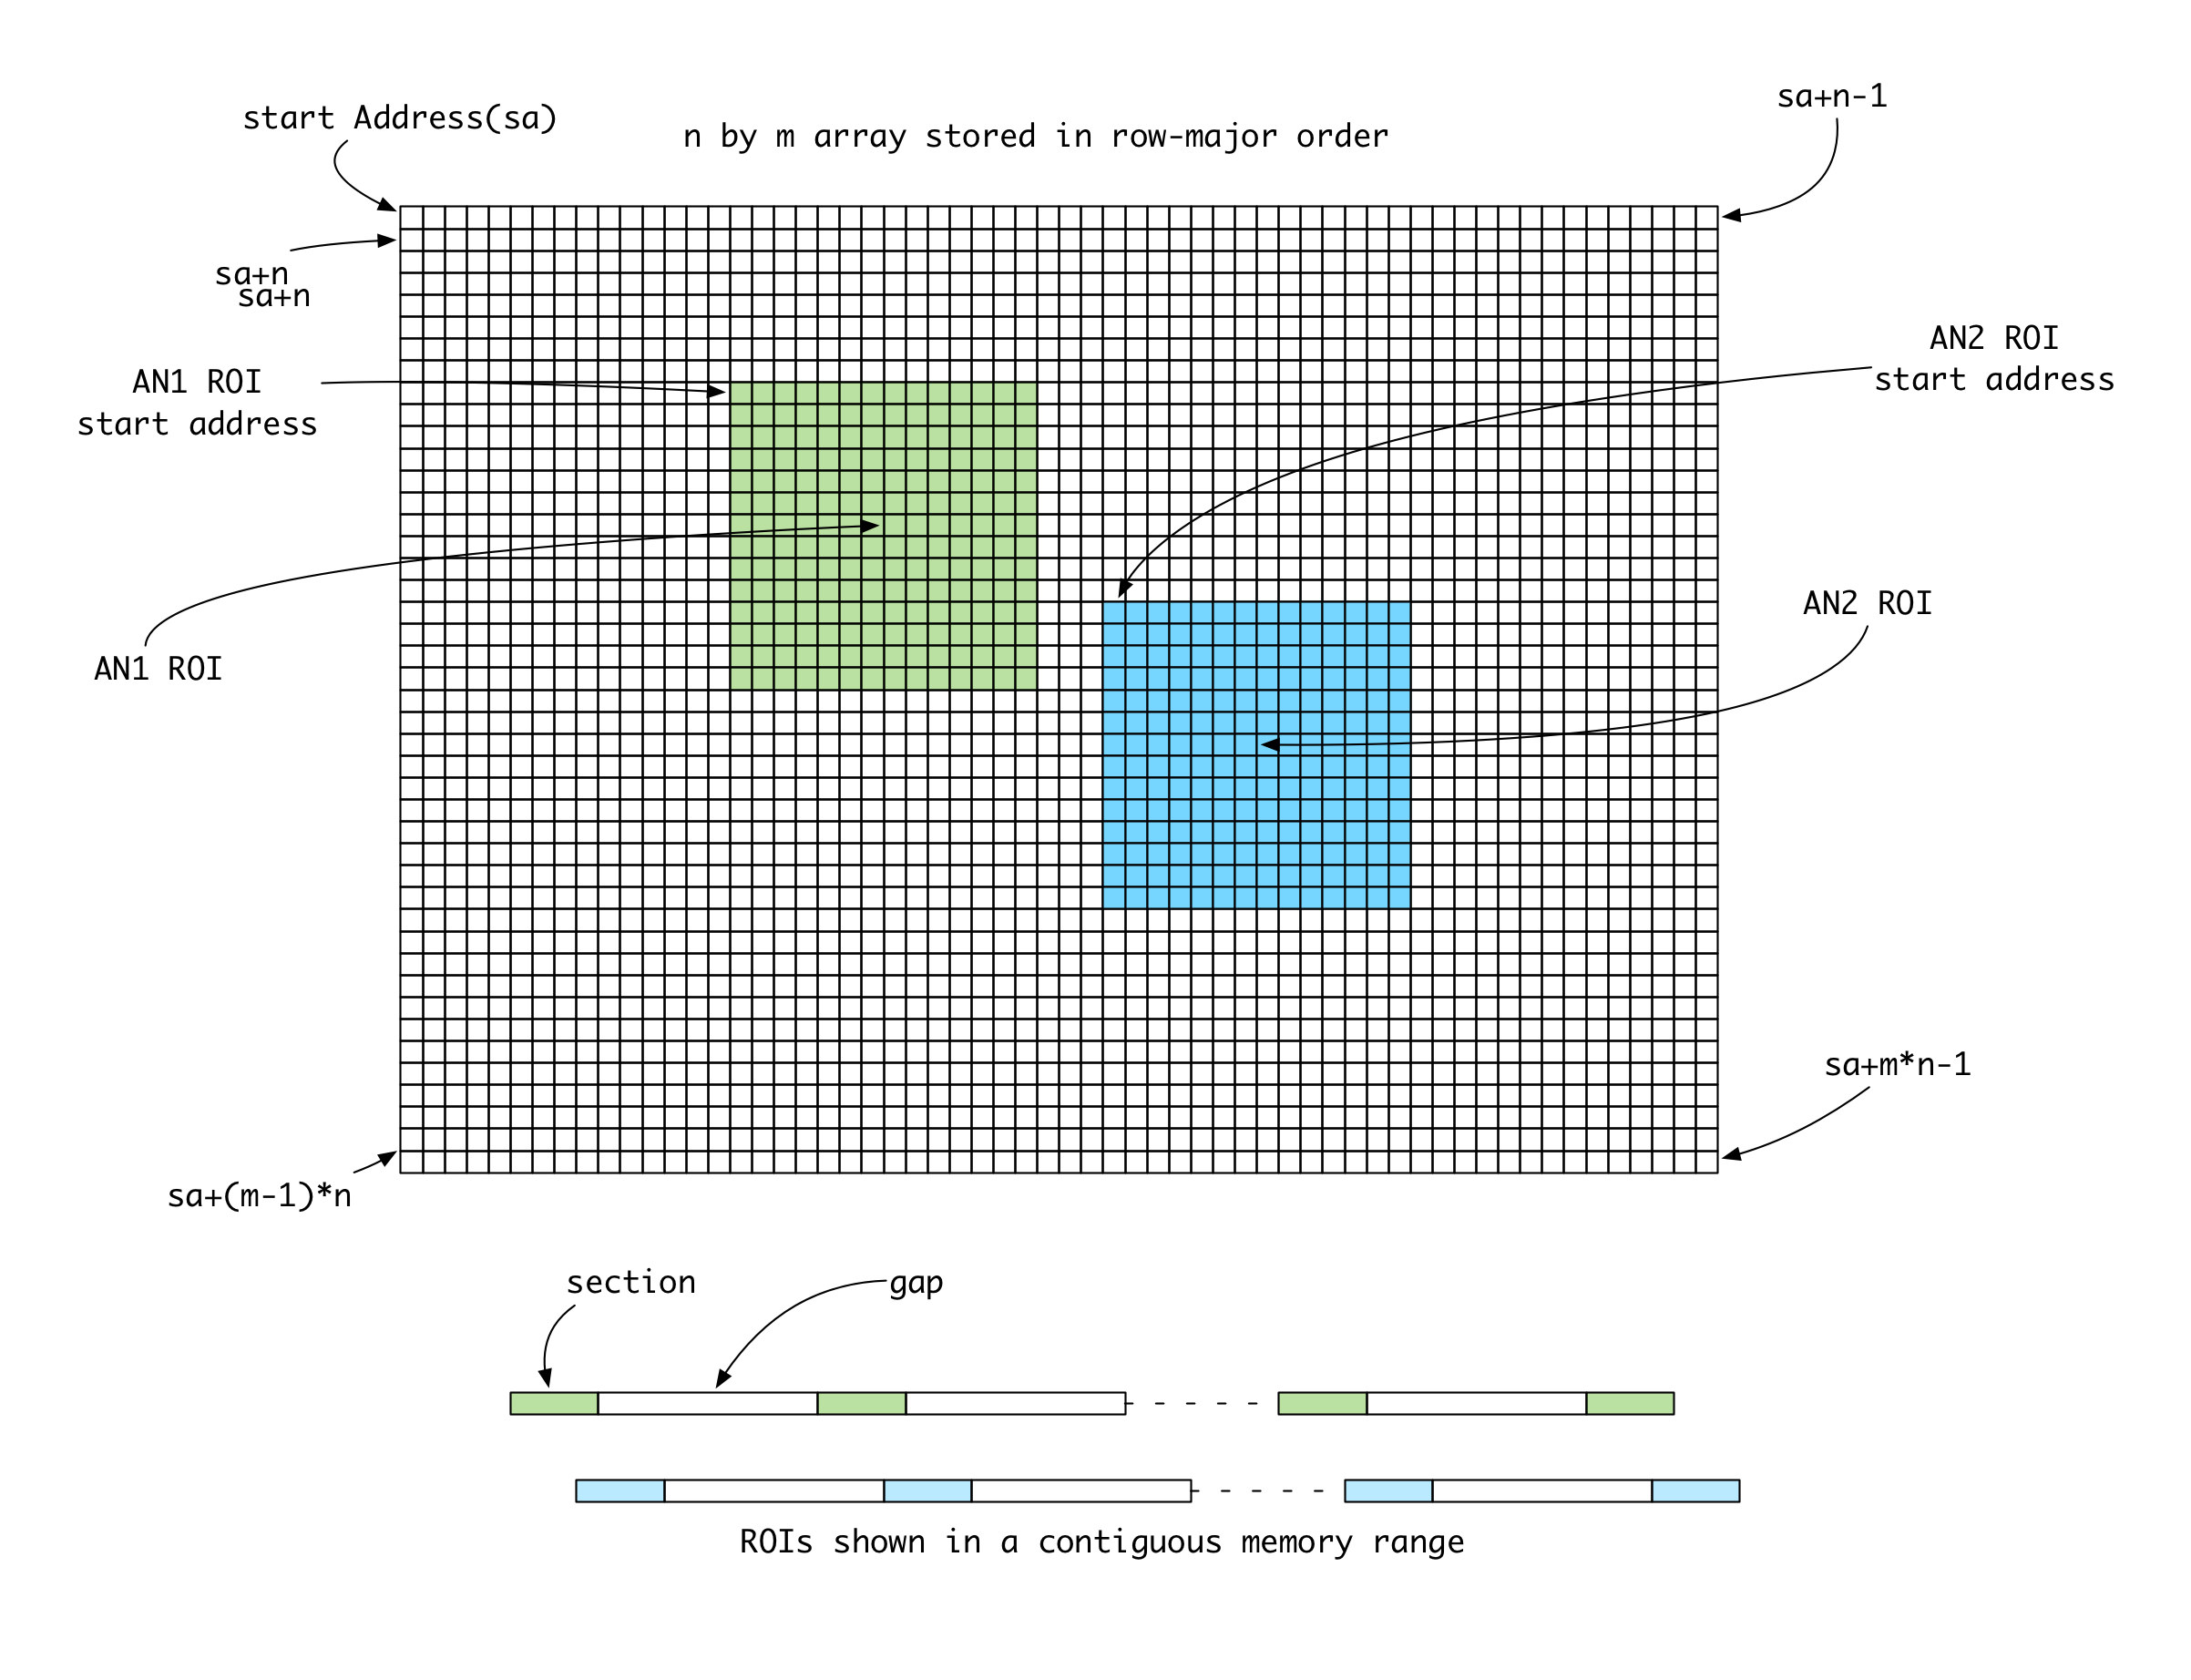
\includegraphics[width=.9\linewidth]{roiStorage.jpg}}
}
\caption{ROI Storage}
\label{fig:roiStorage}
\end{figure}

The various connection weights are stored in multiple contiguous sections. However, its not possible to arrange the input in such a way that each \acp{an} \ac{roi} can be stored in contiguous memory locations. 
A typical \ac{roi} arrangement is shown in figure \ref{fig:roiStorage}. Assuming the input array is stored in row-major order, an \ac{roi} is drawn from disjoint sections of memory. 
These disjoint sections contain a number of \ac{an} states, in this case 14 and the sections are separated by a gap of a number of memory addresses. 
When the parameters are accessed when performing a particular operation, the memory controller within the manager must be informed of the start address and the lengths of the sections and gaps. 
In practice groups of \acp{an} share a common \ac{roi} so often when reading an \ac{roi} from the \ac{dram} it is broadcast across a group of execution lanes.

The read efficiency problem is solved by again taking advantage of the \ac{dram}s banks and pages.

This work proposes a data structure to describe these \ac{roi} storage locations.

Although disparate groups of \acp{an} may have a different start addresses for their \ac{roi}, a commonality is observed in the \ac{roi} section lengths and gaps. So for each \ac{an} group, the groups \ac{roi} starting address is stored along with a pointer to a common set of section length/gaps. This structure is termed a storage descriptor.

This storage descriptor contains, amongst other things the start address of the \ac{roi} and a pointer to a section/gap descriptor. Many storage descriptors point to a common section/gap descriptor. This avoids having to have a unique section/gap descriptors for each \ac{an} group.

Figure \ref{fig:storageDescriptor} shows the structure of the storage descriptor. The \ac{sod}, \ac{mod} and \ac{eod} are used to delineate each storage descriptor in memory.

\begin{figure}[!t]
\centering
\captionsetup{justification=centering}
\captionsetup{width=.9\linewidth}
\centerline{
\mbox{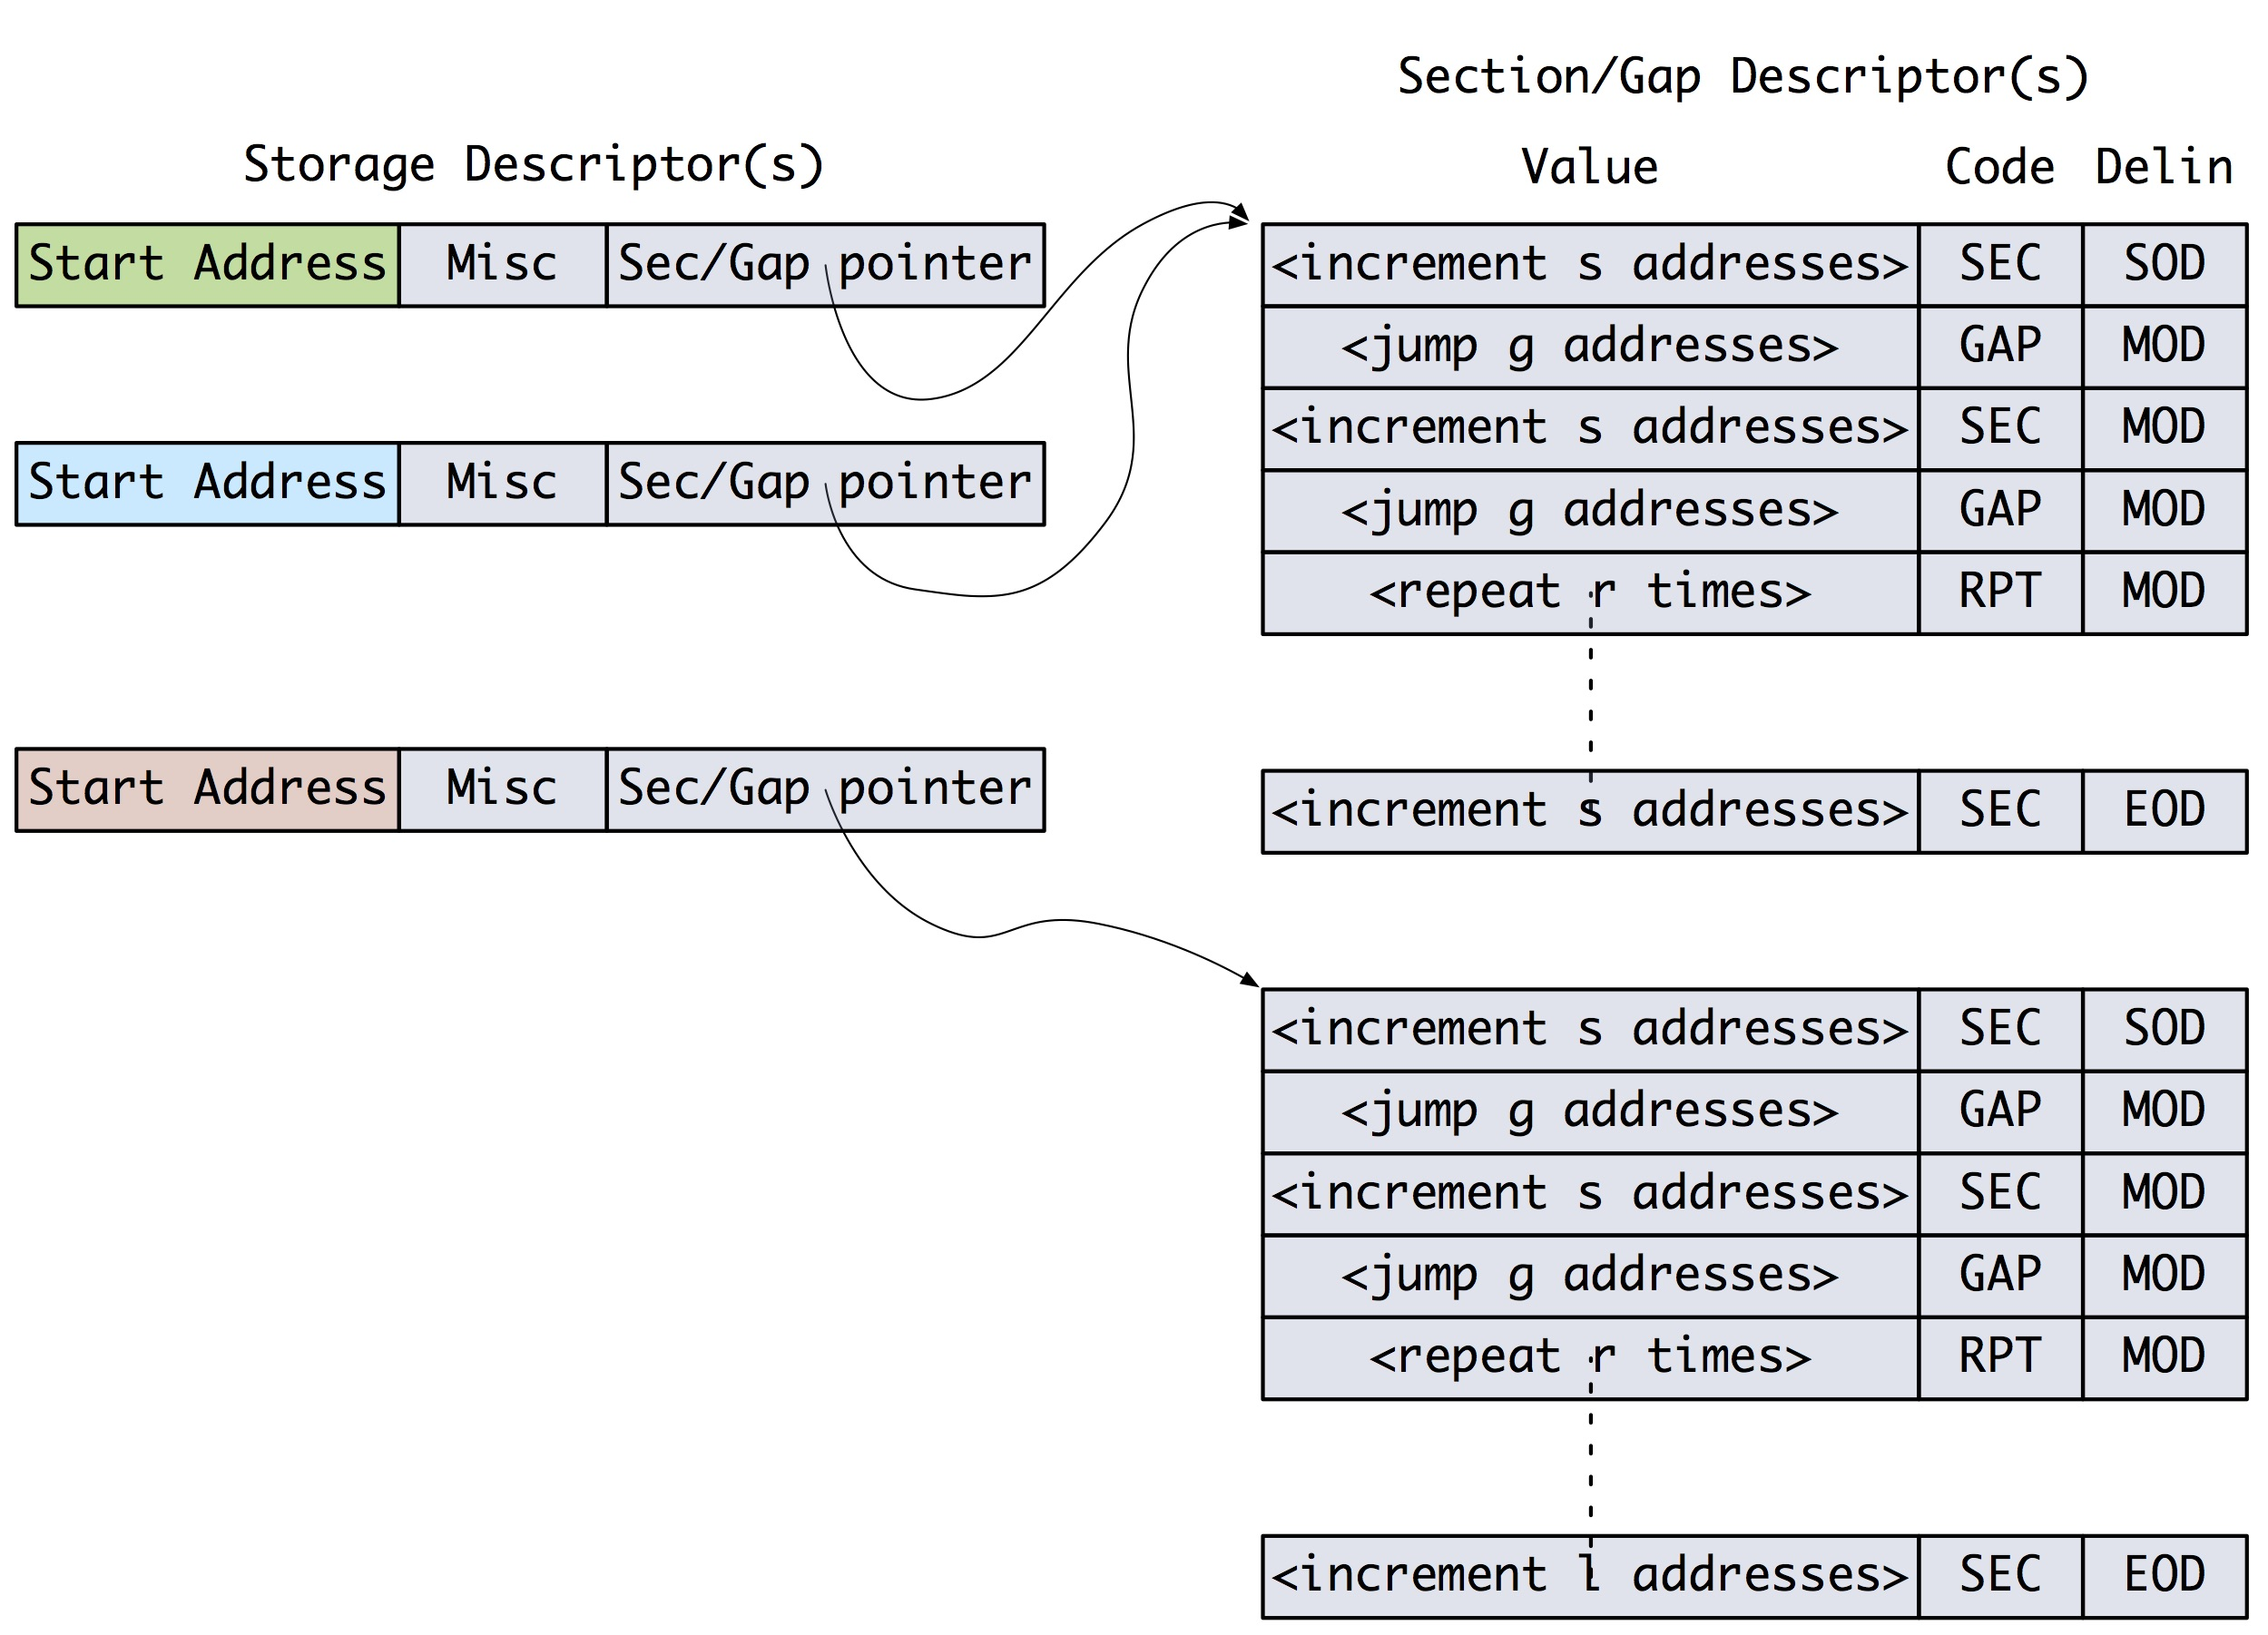
\includegraphics[width=.9\linewidth]{storageDesc.jpg}}
}
\caption{Storage Descriptor}
\label{fig:storageDescriptor}
\end{figure}

% ----------------------------------------------------------------------------------------------------
\subsubsection{Writing \ac{an} state results to memory}
\label{sec:writingANStates}

When the \ac{pe} has processed the group of \acp{an}, the new \ac{an} states are sent back to the manager and stored to \ac{dram} in the row-major array format described earlier.
\iffalse
A significant difference taken advantage of is that for any given operation, the system is writing far less than is being read. For example, the \ac{roi} and parameters are usually vectors that will typically exceed 100 elements and in many cases much higher. When an operation is complete, in almost all cases one word per lane is writen back to main memory. 
Now that sounds like writing back has a very small impact on performance but with \ac{dram}s thats not always true.
\fi
When an operation is complete, in almost all cases one word per lane is writen back to \ac{dram}.
Considering a \ac{dram} page contains 128 words, the system typically writes a $4$th of a page and this is a relatively inefficient use of \ac{dram} bandwidth. 
However, the pre-synaptic fanin typically far exceeds 100 elements and in the baseline \ac{an} shown in table \ref{tab:Baseline Layer Configuration} the average fanin is \num 1650.
So the write to read ratio is very high and the inefficient write has little impact on the overall performance.

As discussed in section \ref{sec:Inter-Manager Communication} in many cases the results have to be provided not only to the local \ac{ssc} \ac{dram} but also to other \acp{ssc} memory. 
This is handled by examining the write storage descriptors and if at least one storage descriptor address references another \acp{ssc} memory, all the write storage descriptors in the instruction are included in the \ac{noc} packet (see figure \ref{fig:NoC packet format}).

% ----------------------------------------------------------------------------------------------------
% ----------------------------------------------------------------------------------------------------
\iffalse
\section{PE Operations}
\label{sec:PE Operations}

% ----------------------------------------------------------------------------------------------------
\subsection{Streaming Operations (\ac{stop})}
\label{sec:streamingOps}
The operations performed by the \ac{stop} are primarily multiple-accumulate with a transfer to the \ac{simd} or to local memory.

Even though the baseline system focuses on the \ac{an} multiply-accumulate followed by a ReLu activation function, the system has built in flexibility into the \ac{stop} function to allow other functions to be added

In most cases, the \ac{stop} module will operate on the \ac{an} state and weights provided by the manager and provide the result to the \ac{simd}.
% ----------------------------------------------------------------------------------------------------
\subsection{SIMD}
\label{sec:SIMD}

The \ac{simd} is a 32-lane processor with some builtin special functions, such as the ReLu operation.

The \ac{simd} will take the result provided by the \ac{stop} and perform a ReLu. The result will, in most cases, then transmitted back to the manager.

% ----------------------------------------------------------------------------------------------------
\subsection{Configuration}
\label{sec:peConfiguration}

To configure these operations, two pointers are sent to the \ac{pe}. These pointers index into a small local memory which provides a program counter (\ac{pc}) to the function to be performed by the \ac{simd} and a configuration entry for the operation to be performed by the \ac{stop}.

The \ac{pe} is able to perform its operation concurrently on 32-lanes. However, there are cases when less than 32-lanes will be employed. This may occur if the number of \acp{an} being processed is not modulo-32. In this case, the manager provides the number of lanes being processed for any given operation. In addition, the length of the vector of operands is also sent by the manager to the \ac{pe}.
\fi

\subsection{Configuration Instruction}
\label{sec:Configuration Instruction}

The configuration instruction is used to :
\begin{itemize}
  \lbbcleanspace
    \item Data transfer
    \begin{itemize}
      \item Download Instructions from host to \ac{ssc} manager instruction memory
      \item Download Sync group data from host to \ac{ssc} manager 
      \item Download \ac{ann} parameters and input from host to \ac{ssc} memory
      \item Upload \ac{ann} output to host from \ac{ssc} memory
    \end{itemize}
  \item System synchronization
    \begin{itemize}
      \item Send a sync message to a group of \acp{ssc}
      \item Wait for sync message from a group of \acp{ssc} or host
      \item Pause instruction fetch
      \item Flush \ac{pe} operations
    \end{itemize}
\end{itemize}

The configuration instruction contains one descriptor and there are two configuration types which are characterized by the descriptor contents.

The data transfer configuration instruction is shown in figure \ref{fig:Data transfer instruction} and the descriptor is a 2-tuple with a data option type and a storage option type.
The sync configuration instruction is shown in figure \ref{fig:Sync instruction} and the descriptor is a 1-tuple with a sync option type.

\begin{figure}
\centering
  \begin{subfigure}{.85\textwidth}
    \centering
    \mbox{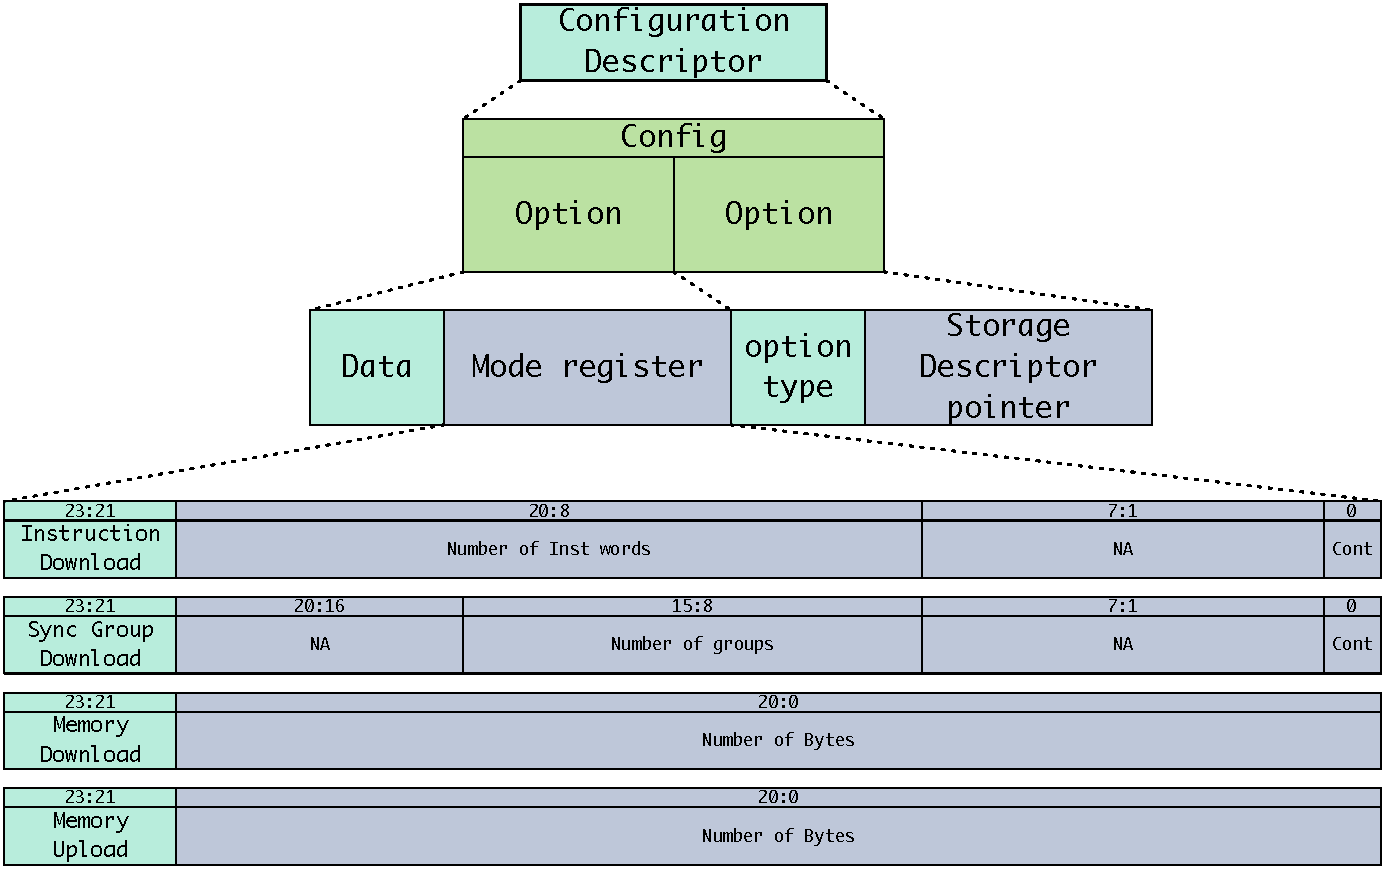
\includegraphics[width=1\linewidth]{dataTransferInstruction}}
    \captionsetup{justification=centering, skip=6pt}
    \caption{Data transfer instruction }
    \label{fig:Data transfer instruction}
  \end{subfigure}%

\bigskip

  \vspace{-35pt}
  \begin{subfigure}{0.85\textwidth}
    \centering
    \vspace{40pt}
    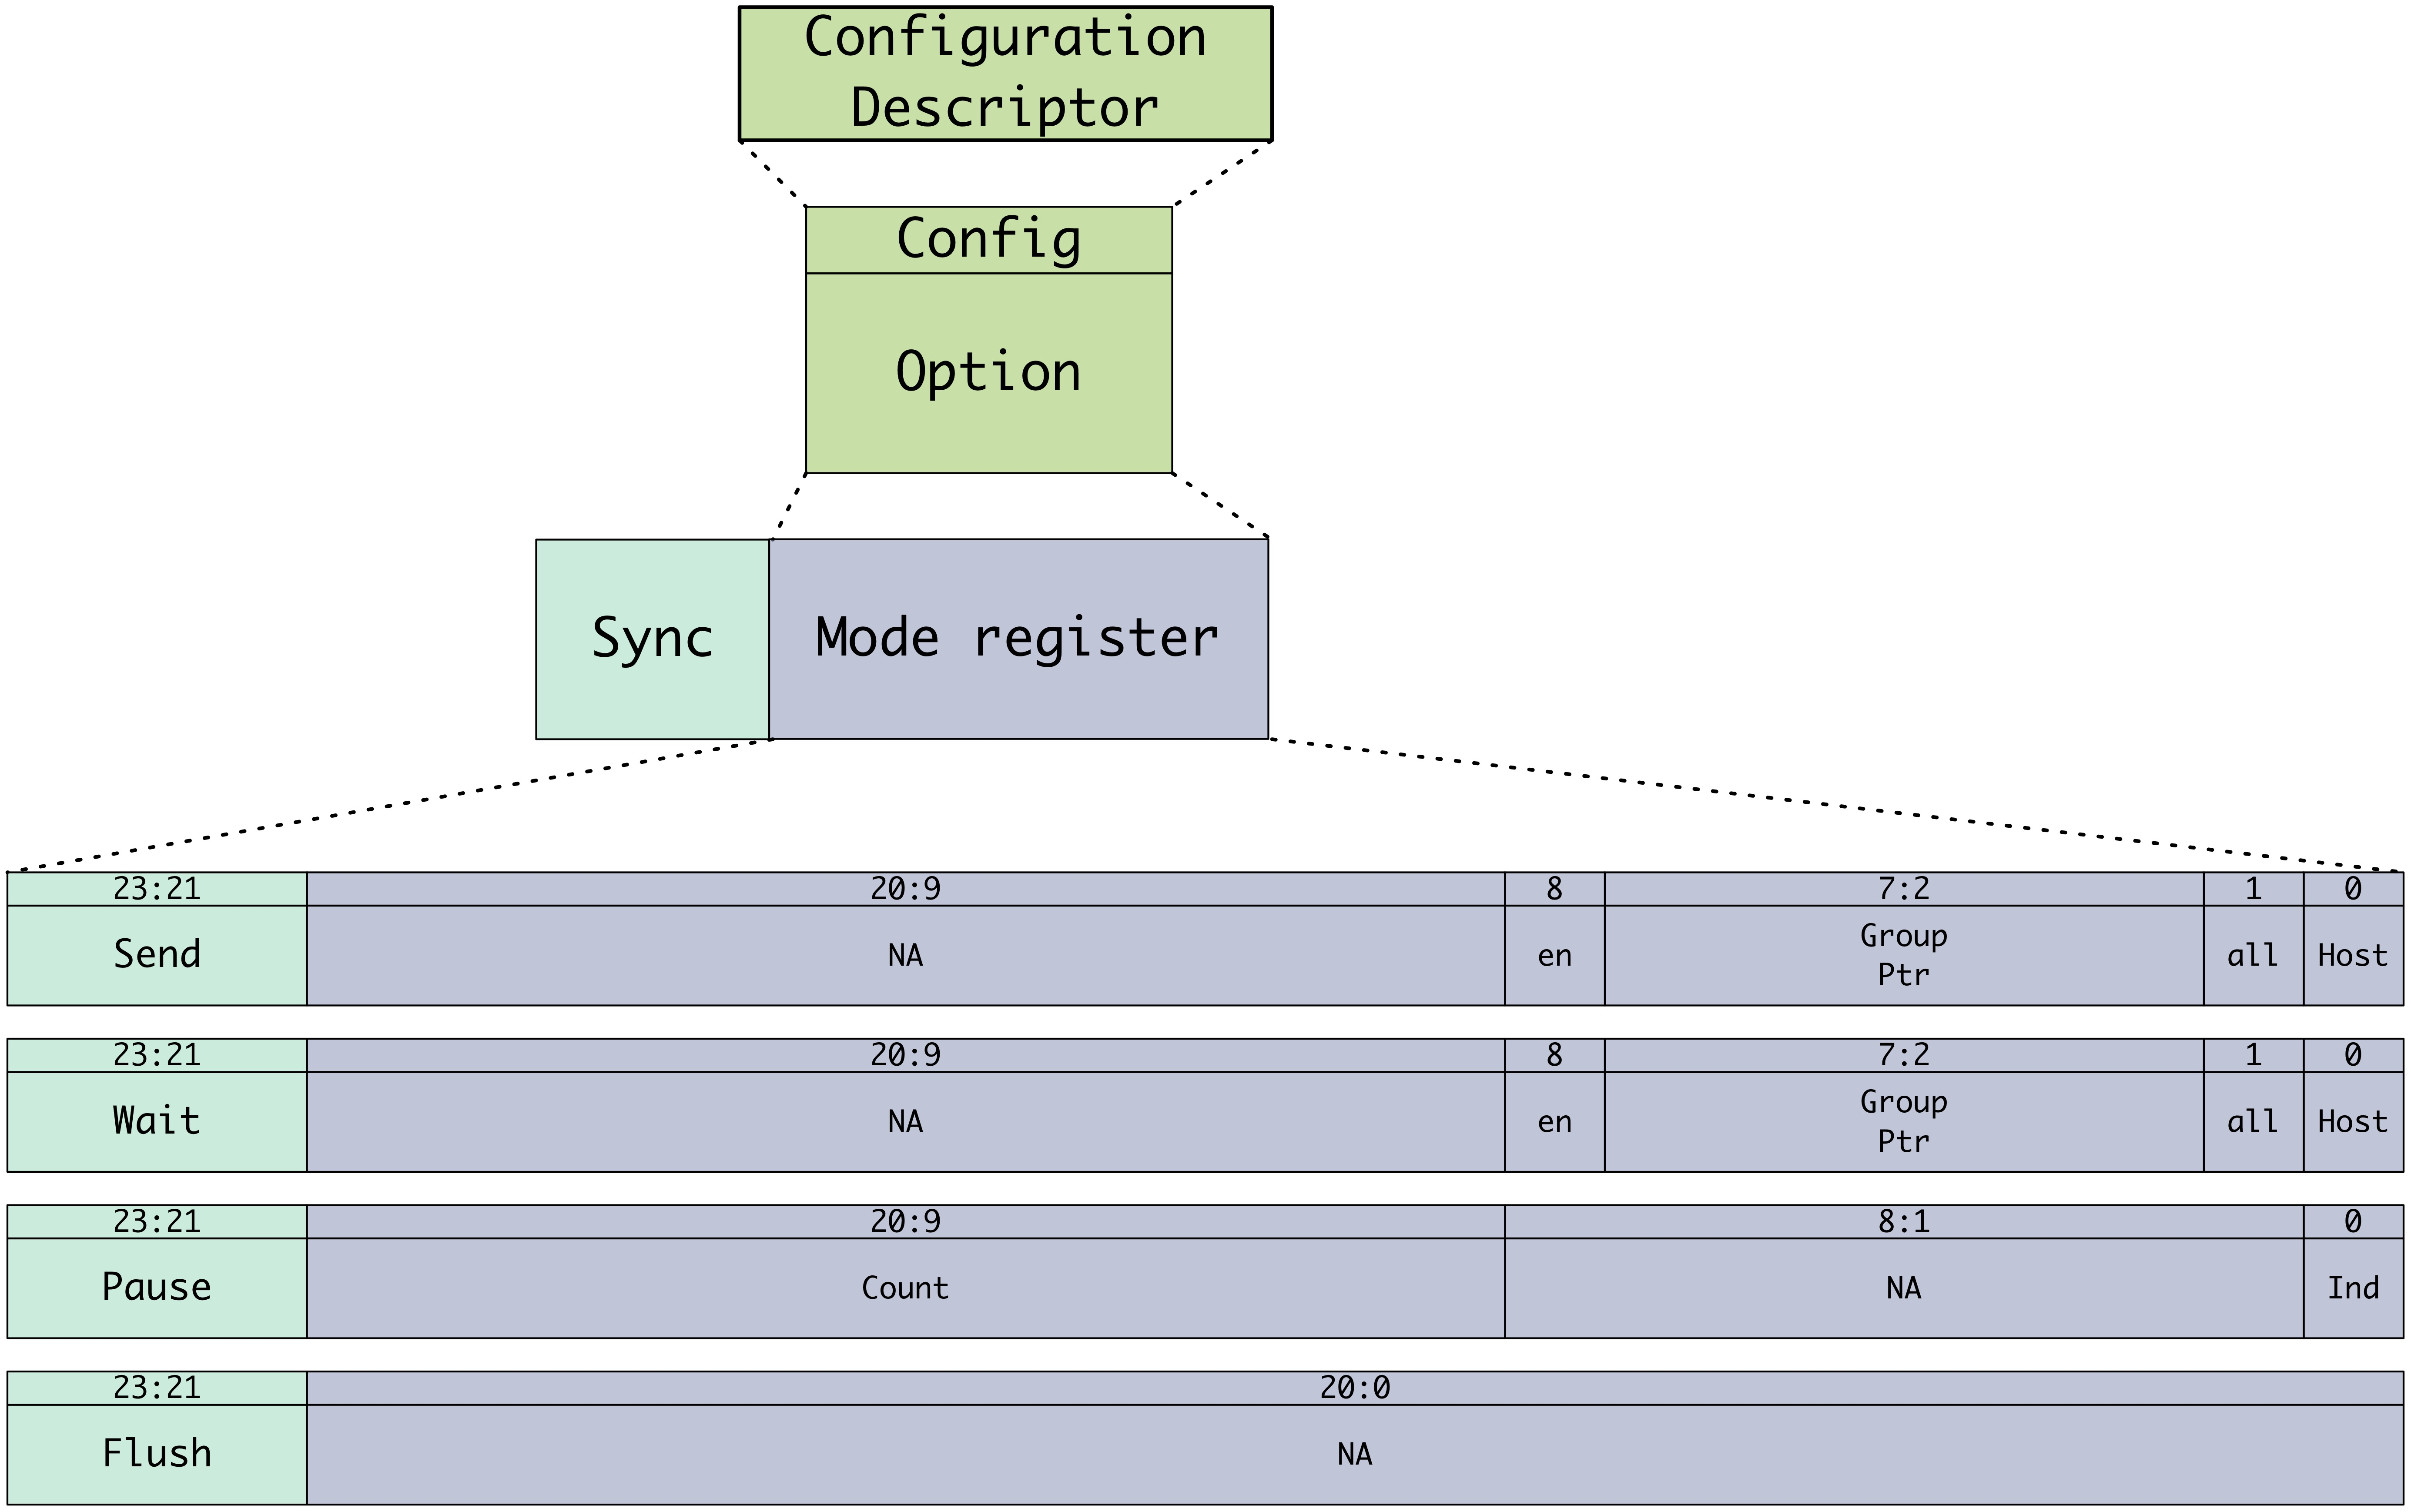
\includegraphics[width=1\textwidth]{syncInstruction}
    \captionsetup{justification=centering, skip=10pt}
    \caption{Sync instruction }
    \label{fig:Sync instruction}
  \end{subfigure}%
%\vspace{-10pt}
\captionsetup{justification=centering, skip=16pt}
\caption{Configuration Instruction types}
\label{fig:Configuration Instruction types}
\end{figure}

The data option value contains a mode register \cite{micron_ddr3} which defines the type of data transfer along with information to aid the transfer. The storage option type contains a storage descriptor pointer which specifies the address of the 
The data transfer instruction ty is broken into a data instruction and a sync instruction.

\subsubsection{Data Transfer Instruction}
\label{sec:Data Transfer Instruction}

The first of the option elements is a data option whose value contains a mode register.
There are currently four mode registers defined, an instruction download register, a sync group downlaod register, a memory downlaod register and a memory upload register.
The contents of the mode register specify the type of transfer, the size of the transfer and some additional flags.
When transferring to or from memory, an additional descriptor element contains a storage descriptor defining where the data should read or written.

\subsubsection{Sync Instruction}
\label{sec:Data Transfer Instruction}

The option element is a sync option whose value contains a mode register.
There are currently four mode registers defined, a send, wait, pause and a flush register.
The contents of the send and wait mode register specify the group of \acp{ssc} to be synchronized. 
The send causes a sync \ac{noc} packet to be sent to all \acp{ssc} in the group.
The wait causes the manager to wait for a \ac{noc} sync packet to be received from all \acp{ssc} in the group.
The pause mode register cause the instruction fetch logic to pause the specified number of clock cycles.
The flush mode register cause the instruction fetch logic to wait for all outstanding \ac{pe} operations to be returned before continuing.

\subsection{Multiple Instruction Functions}
\label{sec:Multiple Instruction Functions}

When instructions or data is downloaded, in some cases there are tasks in the system that must be performed by chaining instructions together.
This is the case when downloading the \ac{pe} operation pointers and the \ac{simd} instructions.
In these cases, the host will have to first download the data to the \ac{ssc} local \ac{dram} in conjunction with a \ac{ssc} configuration download instruction.
The data is then transferred to the \ac{pe} using an operation instruction with the \ac{stop} configured as a \ac{nop} so the data will pass through the \ac{stop} with the small local \ac{sram} as the target. 
The \ac{pe} controller will then transfer the contents of the \ac{sram} to \ac{simd} instruction memory or the operation pointer memory.
As an example, loading the \ac{simd} instruction memory requires the procedure described in algorithm \ref{alg:Load SIMD Instruction memory}.

\begin{algorithm}
\caption{Load SIMD Instruction memory}
\label{alg:Load SIMD Instruction memory}
\begin{algorithmic}[1]
    %      inst       desc
    \State{// last compute instruction}
    \State \makebox[1.05cm][r]{COM:[}\makebox[0.25cm][r]{[}\makebox[0.85cm][r]{  op}\makebox[0.15cm][l]{:}\makebox[0.15cm][r]{[}\makebox[1.00cm][r]{stOp:}\makebox[1.25cm][l]{fpmac}\makebox[0.25cm][r]{,}\makebox[1.00cm][r]{simd:}\makebox[0.80cm][l]{relu }\makebox[0.25cm][r]{,}\makebox[1.65cm][r]{numop0:}\makebox[0.75cm][l]{<n>}\makebox[0.25cm][r]{,}\makebox[1.65cm][r]{numop1:}\makebox[1.00cm][l]{<n>  }\makebox[0.25cm][r]{]} \\
           \makebox[1.05cm][r]{     }\makebox[0.25cm][r]{[}\makebox[0.85cm][r]{  mr}\makebox[0.15cm][l]{:}\makebox[0.15cm][r]{[}\makebox[1.00cm][r]{ tgt:}\makebox[1.25cm][l]{std0 }\makebox[0.25cm][r]{,}\makebox[1.00cm][r]{txfr:}\makebox[0.80cm][l]{bcast}\makebox[0.25cm][r]{,}\makebox[1.65cm][r]{ lanes:}\makebox[0.75cm][l]{<l>}\makebox[0.25cm][r]{,}\makebox[1.65cm][r]{  StoD:}\makebox[1.00cm][l]{<ptr>}\makebox[0.25cm][r]{]} \\
           \makebox[1.05cm][r]{     }\makebox[0.25cm][r]{[}\makebox[0.85cm][r]{  mr}\makebox[0.15cm][l]{:}\makebox[0.15cm][r]{[}\makebox[1.00cm][r]{ tgt:}\makebox[1.25cm][l]{std1 }\makebox[0.25cm][r]{,}\makebox[1.00cm][r]{txfr:}\makebox[0.80cm][l]{vec  }\makebox[0.25cm][r]{,}\makebox[1.65cm][r]{ lanes:}\makebox[0.75cm][l]{<l>}\makebox[0.25cm][r]{,}\makebox[1.65cm][r]{  StoD:}\makebox[1.00cm][l]{<ptr>}\makebox[0.25cm][r]{]} \\
           \makebox[1.05cm][r]{     }\makebox[0.25cm][r]{[}\makebox[0.85cm][r]{  mw}\makebox[0.15cm][l]{:}\makebox[0.15cm][r]{[}\makebox[1.00cm][r]{ src:}\makebox[1.25cm][l]{stu  }\makebox[0.25cm][r]{,}\makebox[1.00cm][r]{txfr:}\makebox[0.80cm][l]{vec  }\makebox[0.25cm][r]{,}\makebox[1.65cm][r]{ lanes:}\makebox[0.75cm][l]{<l>}\makebox[0.25cm][r]{,}\makebox[1.65cm][r]{  StoD:}\makebox[1.00cm][l]{<ptr>}\makebox[0.25cm][r]{,}\makebox[1.00cm][r]{  StoD:}\makebox[1.00cm][l]{<ptr>}\makebox[0.25cm][r]{]} 
\\
    \State{//---------------------------------------- Start download ---------------------------------------- }
    \State{// make sure all compute instruction are complete}
    \State \makebox[1.05cm][r]{CFG:[}\makebox[0.25cm][r]{[}\makebox[0.85cm][r]{ cfg}\makebox[0.15cm][l]{:}\makebox[0.15cm][r]{[}\makebox[1.00cm][r]{sync:}\makebox[0.25cm][r]{[}\makebox[1.75cm][r]{flush}\makebox[0.25cm][r]{]}\makebox[0.25cm][r]{]}
    \State \makebox[1.05cm][r]{CFG:[}\makebox[0.25cm][r]{[}\makebox[0.85cm][r]{ cfg}\makebox[0.15cm][l]{:}\makebox[0.15cm][r]{[}\makebox[1.00cm][r]{sync:}\makebox[0.25cm][r]{[}\makebox[1.75cm][r]{send:}\makebox[0.25cm][r]{[}\makebox[1.00cm][l]{host }\makebox[0.25cm][r]{]}\makebox[0.25cm][r]{]}\makebox[0.25cm][r]{]}
    \State \makebox[1.05cm][r]{CFG:[}\makebox[0.25cm][r]{[}\makebox[0.85cm][r]{ cfg}\makebox[0.15cm][l]{:}\makebox[0.15cm][r]{[}\makebox[1.00cm][r]{sync:}\makebox[0.25cm][r]{[}\makebox[1.75cm][r]{wait:}\makebox[0.25cm][r]{[}\makebox[1.00cm][l]{host }\makebox[0.25cm][r]{]}\makebox[0.25cm][r]{]}\makebox[0.25cm][r]{]}
    \State{// Host sends release}
\\
    \State{// Host starts simd instruction download to SSC memory}
    \State{// Next SSC instruction prepares wr\textunderscore cntl for data from Host}
    \State \makebox[1.05cm][r]{CFG:[}\makebox[0.25cm][r]{[}\makebox[0.85cm][r]{ cfg}\makebox[0.15cm][l]{:}\makebox[0.15cm][r]{[}\makebox[1.00cm][r]{data:}\makebox[0.25cm][r]{[}\makebox[1.75cm][r]{mem\textunderscore dn:}\makebox[1.00cm][l]{<m>}\makebox[0.25cm][r]{,}\makebox[1.65cm][r]{  StoD:}\makebox[1.00cm][l]{<ptr>}\makebox[0.25cm][r]{]}
    \State \makebox[1.05cm][r]{CFG:[}\makebox[0.25cm][r]{[}\makebox[0.85cm][r]{ cfg}\makebox[0.15cm][l]{:}\makebox[0.15cm][r]{[}\makebox[1.00cm][r]{sync:}\makebox[0.25cm][r]{[}\makebox[1.75cm][r]{pause:}\makebox[0.25cm][r]{[}\makebox[1.00cm][l]{ind }\makebox[0.25cm][r]{]}\makebox[0.25cm][r]{]}\makebox[0.25cm][r]{]}
    \State{// fetch paused waiting for release, wr\textunderscore cntl ready for Host data}
    \State{// wr\textunderscore cntl releases fetch when data transfer complete}
    \State \makebox[1.05cm][r]{COM:[}\makebox[0.25cm][r]{[}\makebox[0.85cm][r]{  op}\makebox[0.15cm][l]{:}\makebox[0.15cm][r]{[}\makebox[1.00cm][r]{stOp:}\makebox[1.25cm][l]{ld\textunderscore simd}\makebox[0.25cm][r]{,}\makebox[1.00cm][r]{simd:}\makebox[0.80cm][l]{nop  }\makebox[0.25cm][r]{,}\makebox[1.65cm][r]{numop0:}\makebox[0.75cm][l]{<m>}\makebox[0.25cm][r]{]} \\
           \makebox[1.05cm][r]{     }\makebox[0.25cm][r]{[}\makebox[0.85cm][r]{  mr}\makebox[0.15cm][l]{:}\makebox[0.15cm][r]{[}\makebox[1.00cm][r]{ tgt:}\makebox[1.25cm][l]{std0}\makebox[0.25cm][r]{,}\makebox[1.00cm][r]{txfr:}\makebox[0.80cm][l]{bcast}\makebox[0.25cm][r]{,}\makebox[1.65cm][r]{ lanes:}\makebox[0.75cm][l]{1}\makebox[0.25cm][r]{,}\makebox[1.65cm][r]{  StoD:}\makebox[1.00cm][l]{<ptr>}\makebox[0.25cm][r]{]}
    \State{// manager sending instruction data to PE using compute operation with NOPs}
    \State{// flush PE to ensure instruction data complete}
    \State \makebox[1.05cm][r]{CFG:[}\makebox[0.25cm][r]{[}\makebox[0.85cm][r]{ cfg}\makebox[0.15cm][l]{:}\makebox[0.15cm][r]{[}\makebox[1.00cm][r]{sync:}\makebox[0.25cm][r]{[}\makebox[1.75cm][r]{flush}\makebox[0.25cm][r]{]}\makebox[0.25cm][r]{]}
    %\State \makebox[1.05cm][r]{CFG:[}\makebox[0.25cm][r]{[}\makebox[0.85cm][r]{ cfg}\makebox[0.15cm][l]{:}\makebox[0.15cm][r]{[}\makebox[1.00cm][r]{sync:}\makebox[0.25cm][r]{[}\makebox[1.75cm][r]{send:}\makebox[0.25cm][r]{[}\makebox[1.00cm][l]{host }\makebox[0.25cm][r]{]}\makebox[0.25cm][r]{]}\makebox[0.25cm][r]{]}
    %\State \makebox[1.05cm][r]{CFG:[}\makebox[0.25cm][r]{[}\makebox[0.85cm][r]{ cfg}\makebox[0.15cm][l]{:}\makebox[0.15cm][r]{[}\makebox[1.00cm][r]{sync:}\makebox[0.25cm][r]{[}\makebox[1.75cm][r]{wait:}\makebox[0.25cm][r]{[}\makebox[1.00cm][l]{host }\makebox[0.25cm][r]{]}\makebox[0.25cm][r]{]}\makebox[0.25cm][r]{]}
    \State{//---------------------------------------- end of download ---------------------------------------- }
\\
    \State{// continue with compute instructions}
    \State \makebox[1.05cm][r]{COM:[}\makebox[0.25cm][r]{[}\makebox[0.85cm][r]{  op}\makebox[0.15cm][l]{:}\makebox[0.15cm][r]{[}\makebox[1.00cm][r]{stOp:}\makebox[1.25cm][l]{fpmac}\makebox[0.25cm][r]{,}\makebox[1.00cm][r]{simd:}\makebox[0.80cm][l]{relu }\makebox[0.25cm][r]{,}\makebox[1.65cm][r]{numop0:}\makebox[0.75cm][l]{<n>}\makebox[0.25cm][r]{,}\makebox[1.65cm][r]{numop1:}\makebox[1.00cm][l]{<n>  }\makebox[0.25cm][r]{]} \\
           \makebox[1.05cm][r]{     }\makebox[0.25cm][r]{[}\makebox[0.85cm][r]{  mr}\makebox[0.15cm][l]{:}\makebox[0.15cm][r]{[}\makebox[1.00cm][r]{ tgt:}\makebox[1.25cm][l]{std0 }\makebox[0.25cm][r]{,}\makebox[1.00cm][r]{txfr:}\makebox[0.80cm][l]{bcast}\makebox[0.25cm][r]{,}\makebox[1.65cm][r]{ lanes:}\makebox[0.75cm][l]{<l>}\makebox[0.25cm][r]{,}\makebox[1.65cm][r]{  StoD:}\makebox[1.00cm][l]{<ptr>}\makebox[0.25cm][r]{]} \\
           \makebox[1.05cm][r]{     }\makebox[0.25cm][r]{[}\makebox[0.85cm][r]{  mr}\makebox[0.15cm][l]{:}\makebox[0.15cm][r]{[}\makebox[1.00cm][r]{ tgt:}\makebox[1.25cm][l]{std1 }\makebox[0.25cm][r]{,}\makebox[1.00cm][r]{txfr:}\makebox[0.80cm][l]{vec  }\makebox[0.25cm][r]{,}\makebox[1.65cm][r]{ lanes:}\makebox[0.75cm][l]{<l>}\makebox[0.25cm][r]{,}\makebox[1.65cm][r]{  StoD:}\makebox[1.00cm][l]{<ptr>}\makebox[0.25cm][r]{]} \\
           \makebox[1.05cm][r]{     }\makebox[0.25cm][r]{[}\makebox[0.85cm][r]{  mw}\makebox[0.15cm][l]{:}\makebox[0.15cm][r]{[}\makebox[1.00cm][r]{ src:}\makebox[1.25cm][l]{stu  }\makebox[0.25cm][r]{,}\makebox[1.00cm][r]{txfr:}\makebox[0.80cm][l]{vec  }\makebox[0.25cm][r]{,}\makebox[1.65cm][r]{ lanes:}\makebox[0.75cm][l]{<l>}\makebox[0.25cm][r]{,}\makebox[1.65cm][r]{  StoD:}\makebox[1.00cm][l]{<ptr>}\makebox[0.25cm][r]{,}\makebox[1.00cm][r]{  StoD:}\makebox[1.00cm][l]{<ptr>}\makebox[0.25cm][r]{]} 
\end{algorithmic}
\end{algorithm}





